%!TEX root = ../thesis.tex
%*******************************************************************************
%*********************************** First Chapter *****************************
%*******************************************************************************

\chapter{Introduction}  %Title of the First Chapter

\ifpdf
    \graphicspath{{Chapter1/Figs/Raster/}{Chapter1/Figs/PDF/}{Chapter1/Figs/}}
\else
    \graphicspath{{Chapter1/Figs/Vector/}{Chapter1/Figs/}}
\fi

% Recent advances in supervised learning problems in machine learning have mainly been driven by the growth in computational power available and the accompanying ability to crunch through ever-larger annotated datasets. However, one truism still holds: \textit{there is never enough annotated data}. Annotating data is expensive: the Penn Treebank, one of the first large-scale annotation efforts in NLP, cost xxx dollars in 1993, and ImageNet, which revolutionised image recognition, cost xxx dollars. In addition, large-scale annotation efforts usually resort to crowdsourcing data collection to inexpert annotators, which often leads to noisy and low-quality data.

% Due to this, weakly or distantly supervised methods, which allow training of a supervised model on large amounts of indirectly labelled data, often lead to large performance increases at the supervised learning task. While many creative and ingenious ways to extract this supervision signal have been published in the literature, it is not always possible to find an amenable source of auxiliary training signal. Even when such a source of signal is hypothesised to exist, it can be hard to make use of it. @@@flesh out this paragraph. 

% What is freely available in limitless quantities is raw unlabelled data. The hard part is making use of this additional data. When the learning problem is how to generate language from some input, seeing this additional data should give the model an idea of how language is structured, and indeed clever ways of making use of large amounts of raw language have lead to improvements in language generation tasks. This can be either done directly in a noisy channel decomposition (@@@cite), or indirectly using a language model reranker, or back-translation.

% Even on tasks where language is on the input side, such as in text classification, seeing unannotated language can give clues about the underlying language data distribution. One common approach is to assume that data which clusters together in some way should have the same label. There are many ways to implement this hypothesis; one example is the transductive SVM @@@cite, which learns a decision boundary which lies away away from clusters in the unsupervised data. Another is graph-based approaches to semi-supervised learning, which construct a graph of the data and propagate label information along the graph @@more citations.

% Another approach is to model the distribution of the data directly in the classifier. If we use a generative rather than a discriminative model, we have access to the model marginal distribution over the data. By matching this to the unannotated data, we can hopefully improve the forward model (i.e. the model that generates the data from the class label), and therefore the classification performance. However, this requires making assumptions about the underlying data generating process, and wrong assumptions here can often lead to pain rather than gain @@@cite. One reason for this is due to overly rigid and inflexible choices of forward distribution: @@@Nigam et al. show that more expressive forward models can lead to better classification accuracies.

% The above approach is related to density estimation, a type of unsupervised learning. Here, the task is to approximate an unknown distribution given a set of samples; typically, models are evaluated by the probability they give unseen examples. In this light, 

% Another prong in the recent progress of supervised learning has been the renaissance of neural network models. These models have shown an incredible ability to scale with increasing amounts of data (@@@cite that NMT vs PBMT paper), in part due to their flexibility in approximating arbitrary functions @@@cite those approximation results. This flexibility extends to learning distributions: neural network-based probabilistic classifiers are currently state-of-the-art in a range of benchmark machine learning tasks. Given this, it is natural to ask whether it is possible to use neural networks to perform density estimation, in the hope of more accurately capturing the empirical data distribution. There are two main ways to approach density estimation, mainly differing in whether one posits the existence of latent variables.

% Generative models without latent variables typically fix a sequential decomposition of the input and use an autoregressive model to estimate the probability of each part conditioned on all previous parts, appealing to the chain rule of probability. While previously practitioners made Markovian assumptions to handle sparsity in parameter estimation, neural sequence models have the ability to capture unbounded dependencies. The rise of such neural models has led to revolutions in tasks like language modelling @@@cite and speech synthesis @@@cite, where there is a natural ordering of the input. Even when no natural ordering exists, fixing an arbitrary order appears to work well: for example, a left-to-right top-down pixel ordering appears to work well for image density estimation @@@cite the PixelRNN papers.

% In contrast, latent variable models use a two stage generative process: first they sample variables from a prior distribution, and then use a learnt likelihood model to transform these sampled variables to the observed output. Examples of these models include (restricted) Boltzmann machines @@@cite, Helmholtz machines and variational autoencoders (VAEs) @@@cite, and generative adversarial networks (GANs) @@@cite. There is great flexibility in the choice of both prior and likelihood: the prior can be structured and learnt on input data, or continuous and imposed in advance. Further, the choice of likelihood model is also open: one can either generate the entire output in one go, bypassing issues with choosing an ordering (helpful for images), or use an autoregressive model for inherently sequential data. Further, posterior inference over the latent variables given an observed input gives a compressed representation of the input, and this representation is often very useful for downstream tasks.

% As mentioned previously, inference in deep latent variable generative models is a central task. However, the flexibility of neural networks comes at a price: it is often difficult to perform exact inference in these models. VAEs solve this problem by instead treating inference as a learning problem, and learn an approximate posterior distribution, also parametrised as a neural network. The inference network is trained jointly with the forward network, on an approximation to the true model likelihood of the observed data. This reduction of inference to learning, which was also presented much earlier in @@@Dayan95, has lead to a renewed interest in generative modelling with flexible neural network likelihoods. 

% A natural extension of pure generative modelling is to ask whether deep generative models can also improve semi-supervised learning. As previously discussed, overly rigid modelling assumptions can lead to decreased classification performance when the model is trained on unlabelled data. However, the increased flexibility of neural networks may mean that deep generative models can more accurately capture the underlying data generating processing. @@@kingma's paper was the first to explore semi-supervised learning with deep generative models, and showed that unsupervised training can indeed improve supervised classification performance on a toy task.

\epigraph{\textit{What I cannot create, I do not understand.}}{Richard Feynman}

At heart, machine learning seeks algorithms and methods to \textit{understand} the world around us. The exact meaning of `understand' can be difficult to pin down: a common operational definition is that `understanding' means transforming some input $X$ to some output $Y$ in a consistent manner. For example, one classic understanding task is \textit{image classification} -- given an image, output a label in a closed class describing the content of the image (see Figure \ref{fig:chap_1_cat} for an example). Another is \textit{question answering}: given a question in English as input, the machine has to output an answer to that question. Here, the output class is open-ended, since the reply to the question can be free-form natural language.

\begin{wrapfigure}{L}{0.48\textwidth}
\centering
    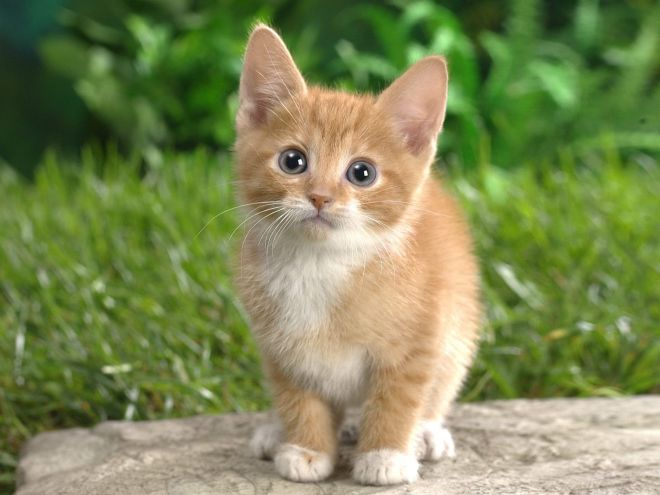
\includegraphics{Chapter1/figs/cat.jpg}
    \caption{Given an image, image classification algorithms try to output a label of the main object in that image. For instance, the label associated with this image is `cat'.}
    \label{fig:chap_1_cat}
    \vspace{-1em}
\end{wrapfigure}

To train such models, the currently predominant approach is \textit{supervised learning}: the model is provided with a dataset of labelled input-output pairs, and is then trained to minimise some error criterion on this dataset. This general paradigm of learning is very flexible, and can be applied to solve many tasks, with a wide variety of models. Indeed, many of the recent flourishings of applied machine learning lean on flexible model classes combined with large amounts of training data \citep{Krizhevsky:12,Wu:16}.

A famous dictum in the early days of statistical learning was `there's no data like more data'\footnote{Bob Mercer, 1985 \citep{Jelinek:05}}, and this trend has continued to the present day. ImageNet \citep{Deng:09}, one of the largest publicly available hand-annotated datasets, comprises \textit{14 million} annotated images collected over 8 years. Further, collecting annotations costs money, and the more specialised the annotation the more expensive it is. For example, SNLI, a large-scale natural language inference understanding dataset, cost around \$55,000 (S Bowman, personal communication) to annotate 500,000 examples; however, the annotation task was relatively straightforward and did not require experts to gather. On the other end of the spectrum, the Penn Treebank \citep{Marcus:93} used 15 graduate linguistics students to annotate 7 million words, and cost roughly \$10 million. A recent annotation effort for French syntax gives a rough figure of \euro{13} per sentence \citep{Martinez-Alonso:16}. Thus, annotating more and more data quickly becomes a time- and money-consuming enterprise, even though raw data is becoming more and more plentiful.

On the other hand, even unlabelled raw data contains much information about the state of the world, and it is conceivable that being able to learn from unlabelled data could benefit machine learning models. Indeed, there is evidence that free-form, undirected observation and interaction with the world (a.k.a. `play') is crucial for child development (\citet{Frost:98} and references therein). Therefore, approaches that can make use of unlabelled data to learn the structure of the world around us hold great potential in unlocking the power of raw data. This subfield of machine learning is called \textit{unsupervised learning}.

One potential approach in this vein is to instead learn to \textit{create} new data which resembles existing data. The core idea is that, just as a successful art forger needs to understand intricately the style of the artist they seek to emulate, so a successful `machine forger' needs to understand the underlying process which gives rise to the observed data. If the observed data comes from natural observations, then this necessarily involves some understanding of the hidden structure of nature.

For example, consider generating images of faces. To be successful at this, a model has to discover that there are independent factors of variation in human faces, such as eye colour and hair colour. In addition, it has to learn the possible eye and hair colours, and what correlations exist between them (such as dark hair predisposing towards darker eyes). Therefore, to do this successfully, the model has to discover the independent features of variation of the data, and how they co-vary; in short, the model has to `carve nature at its joints' \citep{Plato:52}.

In machine learning, models that can generate realistic data points are called \textit{generative models}. They have found wide use in machine learning, both in supervised tasks such as sentiment analysis \citep{Pang:02} and spam email filtering \citep{Pantel:98,Sahami:98}, and on unsupervised structure discovery tasks in fields such as text analysis \citep{Blei:03} and population genetics \citep{Pritchard:00}. Further, due to their ability to generate new data examples, generative models have also been used to explore computational creativity, in domains such as poetry generation \citep{Zhang:14,Ghazvininejad:16,Hopkins:17} and image style transfer \citep{Zhu:17}.

One particular class of generative models are latent variable models. Here, the observed data is assumed to be dependent on unobserved variables. This gives a probabilistic grounding to unsupervised learning techniques such as dimensionality reduction \citep{Tipping:99} and clustering \citep{Gorur:10}. In NLP, classic examples of latent variable models include probabilistic latent semantic analysis (PLSA) \citep{Hofmann:99} and latent Dirichlet analysis (LDA) \citep{Blei:03}. In addition, by encoding assumptions about the generative process in the structure of the latent variables, we can perform structure discovery with latent variable generative models, such as unsupervised dependency parsing \citep{Klein:04,Blunsom:10}. Finally, as latent variable generative models are inherently probabilistic, they gracefully handle output uncertainty well \citep{Kohl:18}.

The core problem of interest with latent variable models is inference on the latent variables given observed data. This is necessary both during learning (for algorithms such as EM \citep{Dempster:77}), and use (i.e. if we want to use the latent variables as data representations). However, calculating the posterior of the latent variables requires calculating the data likelihood. This requires integrating out the latent variables, which is in general infeasible. While closed form expressions for the posterior exist for certain model classes, this imposes harsh constraints on the form of the model, and rules out using interesting likelihood models, and in particular sequence models like recurrent neural networks (see next paragraph). Another option is approximating the integral using a sampling-based algorithm like Markov chain Monte Carlo ; however, this can have high variance, and requires multiple evaluations of the likelihood, which can be expensive. Alternatively, one can try to approximate the posterior with a simpler class of distributions, and try to select the distribution from this class that most closely matches the true posterior -- this approach is known as \textit{variational inference}. However, this approach is inherently suboptimal due to the approximation involved, and an inexpressive class of distributions can result in poor model fit. Further, selecting the optimal approximate posterior requires optimisation, which can be slow for large data sets.

All these reasons have meant that latent variable models, especially in NLP, have used simple likelihood models to keep inference and optimization tractable. However, over recent years, powerful general-purpose models have revolutionised the field of machine learning, and one particular class of models that have (re)gained traction in recent years are neural networks. These biologically inspired models have shown an incredible ability to scale with data \citep{Koehn:17}, in part due to their ability to universally approximate functions \citep{Cybenko:89}. One particularly appealing feature of neural networks is that they allow the parameterisation of complicated distributions, such as over images or sequences, without making the independence assumptions necessary in pre-existing literature.

An illustrative example of this is in the field of \textit{language modelling}, which assigns probabilities to sequences of words. The dominant approach towards language modelling is to use the chain rule of probability to rewrite the probability of a sequence as a product of individual conditional word probabilities, where the conditioning context is the previous words seen. This reduces the problem of learning a sequence predictor into learning a next word predictor.

The prehistory of language modelling was dominated by \textit{n-gram language models} \citep{Jelinek:76,Baker:90}. These use only the most recent $n$ words to guess the next word, and discard any context from further back than this. However, these models are fundamentally limited: human language contains arbitrary length dependencies in constructions like center embedding, and no $n$-gram model can fully capture these interactions. Indeed Noam Chomsky in a series of papers (starting with \citet{Chomsky:56}) argued against n-gram language models as a model for human cognitive processing of language. Neural networks, and in particular recurrent neural networks \citep{Elman:90,Hochreiter:97}, on the other hand, can encode arbitrary length contexts without making any independence assumptions \citep{Mikolov:10,Sundermeyer:12}. Due to this, they currently set the state of the art for language models when evaluated intrinsically using perplexity \citep{Melis:18}, although there is evidence to show that on huge datasets n-gram language models can still achieve competitive performance \citep{Chelba:17}.

% One particularly exciting application of neural networks is as the likelihood function of a generative model. This combination is broadly known as a \textit{deep generative model}. Early work in this area include Boltzmann machines \citep{Ackley:85}, and Helmholtz machines \citep{Dayan:95}. However, these models either require sampling to train, which can be slow, or do not optimise a valid bound on the data (log-)likelihood, which can lead to inconsistent parameter estimation.

Given these spectacular successes, a natural line of enquiry is whether we can combine neural networks and latent variable generative models. As with all neural network research, there is much early work on this area, including (restricted) Boltzmann machines \citep{Hinton:83,Ackley:85,Smolensky:86} and Helmholtz machines \citep{Dayan:95}. However, these models either require sampling to train \citep{Hinton:02,Tieleman:08}, or do not optimise a valid bound on the data log-likelihood \citep{Hinton:95}. Further, the model architectures considered only account for fixed-size outputs, and so previous applications of deep generative models to text still made strong word independence assumptions \citep{Hinton:09}.

Work in this area was revitalised by a central idea published contemporaneously by 3 different groups \citep{Kingma:14,Rezende:14,Titsias:14}. One problem with classic variational inference is that typically the parameters of the approximation to the true posterior were optimised independently for each data point. This results in an inner optimization loop inside the main optimization loop, which can be prohibitively slow for large data sets. However, one can view the optimal variational parameters as a function of the input data, and then try to approximate this function with a neural network. Further, we can train this neural network jointly with the generative model to optimize a valid bound on the data log-likelihood, using low-variance single sample gradient estimates of this bound with the \textit{reparametrization trick}. This combination of model, inference and learning is collectively known as a \textit{variational auto-encoder}, or VAE for short, due to similarities with classical autoencoders.

%This idea showed the way to train generative models of text without making restrictive independence assumptions. In particular, we can now train latent variable generative models with powerful sequence-level RNN likelihood functions, an approach first pioneered in \citet{Bowman:16}. These papers serve as the launching point of my thesis, where I explore applications of latent variable models in various NLP tasks.

The power of the variational autoencoder is that it provides a very general recipe to perform inference and learning in a wide range of generative model architectures. Building on this, \citet{Bowman:16} showed how to train latent variable generative models of text with autoregressive likelihoods, and demonstrated that the latent variables captured global information about the sentences. My thesis continues this line of work, and explores both modelling advances and applications of deep generative models of text.

\section{Thesis contributions}

This thesis contains three main contributions:

\begin{itemize}
    \item In Chapter \ref{chap:chatbot}, I present a latent variable model for generating responses in open-domain conversation. Here, the latent variables are continuous, with a Gaussian prior, and summarise the external unobserved factors that account for variation in reply to a given prompt. I give a brief overview of the history of conversational AI, present my contribution, and motivate why a latent variable model is an intuitive idea for open-domain conversation. I evaluate the diversity of the outputs the model produces compared to baseline approaches towards open-domain dialogue, and present some human evaluation to show that humans prefer the output generated by the latent variable model compared to a baseline.
    
    \item In Chapter \ref{chap:sentencelda} I present an extension to LDA which instead draws entire sentences from the latent topics. Here, the latent variables are discrete, and represent a semantic topic for the sentence. I outline the motivation behind doing so, and also discuss the engineering challenges behind optimising such a model, and how I overcame them. I demonstrate that the resulting model is a very powerful model of documents, with better perplexity scores than a wide range of existing latent-variable baselines. I also perform a qualitative analysis of the topics the model learns, and show that the topics the model learns are semantically coherent as judged by human annotators.
    
    \item In Chapter \ref{chap:amrgeneration}, I present a model for generating a surface form from a semantic representation by generating first a syntactic representation. Here, the latent variable is the syntax, which is a structured discrete latent variable. I show that factorising the model in this way leads to state-of-the-art results in AMR generation as measured by automated metrics. Further, we show that as our model has knowledge of syntax, we can generate syntactically varied realisations of the same underlying semantic form, and that human annotators prefer this variation over variation from a baseline model.
\end{itemize}

\section{Additional work not included in this thesis}

During my PhD, I have had the fortune to work on many topics, some of which did not fit into this thesis. In the interests of completeness, I shall talk briefly about those papers in this section, and try to sketch how they relate to the main theme of my thesis.

\subsection{A joint model for word embedding and word morphology}

\textit{This material first appeared in \citet{Cao:16}}

In this paper, I tackle the problem of word segmentation and word subunit discovery using distributional information. To do this, I propose a model that, given a proposed binary segmentation point in a word, composes the characters to the left and right of the point to obtain a representation of the segmented word. The representations of all possible binary segmentations are then combined with a weighted sum to obtain a representation for the word. The model is trained using the skip-gram with negative sampling objective from \citet{Mikolov:13}: I use  the composed word representations to predict context words. The intuition behind the model is that word segmentations which uncover morphemes give rise to representations which are helpful to predict neighbouring words and are thus upweighted, while random segmentations do not help predict context words and are downweighted. This model can be viewed as performing approximate inference in a latent variable model of context word prediction where the latent variables are proposed word segmentations.

I evaluated the model proposed segmentations against baseline word segmenters, and show that it achieves comparable segmentation accuracies to existing unsupervised morphological analyzers. I further evaluated the quality of the compositional word representations the model learns, and show that they outperform a baseline compositional word representation model on rare morphologically complex words, and also at the task of syntactic analogy solving. Finally, I qualitatively examine word nearest neighbours in embedding space, and show that the model learns both orthographic and semantic similarity.

\subsection{Emergent communication through negotiation}

\textit{This material first appeared in \citet{Cao:18}}

In this paper, I examine the possibility of two agents establishing a communication protocol to enable the division of a shared pool of items, with each agent having a differing value for each item. This is done entirely ground up: the only supervision signal the agents receive is the task reward at the end; that is, the value of the items each agent receives. We examine various forms of communication protocol, and various agent payoffs, and show that if the agents are self-interested (that is, receive reward only according to the items they themselves obtain) and communicate using 'cheap talk' (ungrounded symbols without \textit{a priori} semantics), they cannot learn to solve this task.